\subsection{第一原理計算とデータ科学・機械学習による物質科学研究(河村 光晶)}

% 物質内の原子や電子の微視的なふるまいを何ら経験的なパラメーターを用いずに予測する第一原理計算は、各種スペクトル測定やバルク物理量の測定といった実験と相補的な情報を得ることができ、それらと組み合わせることにより物性発現のメカニズムを詳細に解析することができる。
% %
% 水素分子が単原子触媒に解離吸着し担体基板へと移動する水素スピルオーバーは、水素貯蔵やメタノール、アンモニア等の合成における基本的なステップであるが、水素原子の位置や結合状態を実験で直接測定することは極めて難しい。
% 我々は銅(111)表面におけるパラジウム単原子触媒における水素スピルオーバーの機構を解明するため、長田・吉信らによるX線内核光電子分光実験と第一原理内核電子束縛エネルギー計算手法の協奏による研究を行った~\cite{osada.pccp.24.21705}。
% %X線光電子分光では各元素ごとにスペクトルピークが大きく異なること(特性X線)とそれらのピークが原子の局所的な状況などの影響を受けて変化する(化学シフト)を利用して元素選択的な測定を行うことができる。
% 第一原理原子構造最適化により、解離した水素原子がパラジウム原子近傍の三つの特徴的なサイトに吸着し、それらのサイトが全て占有されると銅基盤へとスピルオーバーする事、それらの占有構造での内核電子束縛エネルギー計算とX線光電子分光実験の結果が矛盾しないことが確かめられた。
% この結果は、表面合金触媒の動作機構を理解しデザインする上での知見となる。

% 温度・圧力等の変化によって物質が電気伝導性を失う金属絶縁体転移は、高温超伝導や強誘電といった特異な物性と深く係っている興味深い相転移現象であるが、その転移の機構は異なっており単純なモデルではなく詳細な解析が必要となる。
% 平井らによって新たに合成されたリン化ルテニウムも金属絶縁体転移を示す物質であり、我々はX線回折実験と第一原理計算によるワニエ関数を用いた解析により、ルテニウムの$d_{xy}$軌道がの三量体化により結合性・反結合性・非結合性の軌道に分裂し、より低い非結合準位と反結合準位にギャップが生じることにより絶縁化が引き起こされることを見出した~\cite{hirai.jacs.144.17857}。

% このように第一原理計算と各種の実験との協奏により、より詳細な物性の解析を行っていくことが可能であるが、一方で未だ合成されていない物質をシミュレーションによって予測し、新たな物質の合成指針とする試みも行っている。
% 我々は物質に数十~百万気圧もの高圧をかけた際の構造が最密充填構造をとる傾向があることに着目し、小正路らによる球充填を指導原理とした構造探索手法による新規四元系水素化物超伝導体の探索を行った~\cite{koshoji.prm.6.114802}。
% そのうち動的安定かつ相安定で合成可能性の高い二つの物質に対して超伝導密度汎関数理論に基づく超伝導転移温度の計算を行ったところ、それらは超伝導を示すことが分かったが、その転移温度は既存の水素化物超伝導体硫化水素の200ケルビンと比べて極端に低く、10ケルビン以下となった。
% その原因は超伝導に寄与する軌道が、硫化水素では原子間の領域に拡がっており格子振動による超伝導増強効果を強く得られるのに対し、新規四元系水素化物では原子位置に局在しており格子振動の影響を受けにくいためであると考えられる(図\ref{kawamura_fig_charge_ef})。
% %
% \begin{figure}[!tb]
%     \begin{center}
%       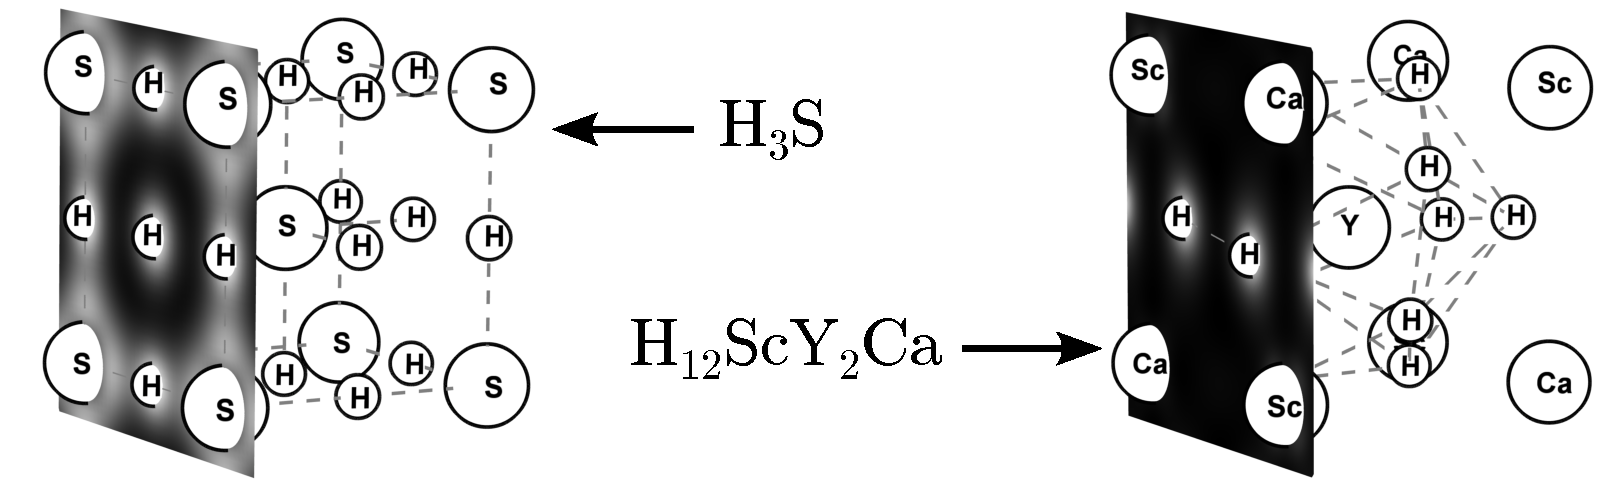
\includegraphics[width=12cm]{Kawamura/charge_ef.pdf}
%       \caption{\label{kawamura_fig_charge_ef}
%         高圧下の硫化水素(左)および新規四元系水素化物(右)の、超伝導に寄与する電子軌道の分布と結晶構造。
%         H、S、Ca、Sc、Yはそれぞれ水素、硫黄、カルシウム、スカンジウム、イットリウム原子を表す。
%         図中の白黒マップは切断面での部分状態密度を表し、明るい部分が大きな値に対応する。}
%     \end{center}
%   \end{figure}
